\documentclass{JAC2003}

%%
%%  Use \documentclass[boxit]{JAC2003}
%%  to draw a frame with the correct margins on the output.
%%
%%  Use \documentclass[acus]{JAC2003}
%%  for US letter paper layout
%%

\usepackage[dvips]{graphicx}
\usepackage{booktabs}

\newcommand{\opal}{\textsc{OPAL}}
\newcommand{\opalt}{\textsc{OPAL-t }}
\newcommand{\opalcycl}{\textsc{OPAL-cycl}}
\newcommand{\opalmap}{\textsc{OPAL-map }}
\newcommand{\opalenv}{\textsc{OPAL-envelop}}

\newcommand{\mad}{\textsc{mad }}
\newcommand{\madnine}{\textsc{mad9 }}
\newcommand{\madninep}{\textsc{mad9p }}
\newcommand{\madeight}{\textsc{mad8 }}

\newcommand{\classic}{\textsc{classic }}
\newcommand{\hfifepart}{\textsc{H5Part }}
\newcommand{\hfifefe}{\textsc{H5FED }}

\renewcommand{\epsilon}{\varepsilon} 
\renewcommand{\vec}[1]{{\bf #1}} 
\newcommand{\dt}[1]{\frac{\partial #1}{\partial t}}
\newcommand{\dtt}[1]{\frac{\partial^2 #1}{\partial t^2}}
\newcommand{\dtvec}[1]{\frac{\partial {\mathbf #1}}{\partial t}}
\newcommand{\dttvec}[1]{\frac{\partial^2 {\mathbf #1}}{\partial t^2}}
\newcommand{\rot}{\vec{\nabla} \wedge }
\renewcommand{\div}{\vec{\nabla} \cdot }

\def\vec#1{\mathbf{#1}}
\def\vecg#1{\boldsymbol{#1}}
\def\norm#1{\| #1 \|} 
\def\tr{^{\!\top}}

\def\curl{{\bf curl}\,}
\def\curlp{{\rm curl}_p\,}
\def\div{{\rm div}\,}
\def\grad{\nabla}
\def\gradp{\nabla_p}
\def\dotp#1#2{\langle#1,#2\rangle}
\def\eps{\varepsilon}

\newcommand{\mat}[1]{\ensuremath{\boldsymbol{#1}}}
\newcommand{\vect}[1]{\ensuremath{\mathbf{#1}}}
\newcommand{\iprod}[2]{\ensuremath{\langle#1,#2\rangle}}
\newcommand{\abs}[1]{\ensuremath{|#1|}}

\newcommand{\Nedelec}{N\'{e}d\'{e}lec}

\newcommand{\id}[1]{\structure{#1}}

\newcommand {\Co}{{\mathbb{C}}}
\newcommand {\Int}{{\mathbb{Z}}}
\newcommand {\Nat}{{\mathbb{N}}}
%
%
\newcommand {\Hcurl}{{H(\mathbf{curl};\Omega)}}
\newcommand {\Hocurl}{{H_0(\mathbf{curl};\Omega)}}
\newcommand {\Hdiv}{{H(\mathrm{div};\Omega)}}
\newcommand {\Hodiv}{{H_0(\mathbf{div};\Omega)}}
%
\renewcommand {\Re}{{\rm I \kern-2pt R}}
\newcommand{\vc}[1]{\mbox{\boldmath $#1$}}
\newcommand {\RM}[1]{\mathrm{#1}}


\newcommand{\bs}[1]{\mathbf #1}

%%
%%   VARIABLE HEIGHT FOR THE TITLE BOX (default 35mm)
%%

\setlength{\titleblockheight}{35mm}

\begin{document}
\title{NUMERICAL STUDY OF BEAM DYNAMICS IN HIGH INTENSITY CYCLOTRONS INCLUDING NEIGHBORING BUNCH EFFECTS}

\author{J. J. Yang \thanks{yangjianjun00@mails.tsinghua.edu.cn}, 
  CIAE, Beijing, 102413, China \&
  Tsinghua University, Beijing, 100084, China\\
  A. Adelmann \thanks{andreas.adelmann@psi.ch},
  M. Humbel,
  M. Seidel,
  PSI, Villigen, CH-5234, Switzerland\\
  T. J. Zhang, 
  CIAE, Beijing, 102413, China\\}


\maketitle

\begin{abstract}
  For high intensity cyclotrons with small turn separation, the single bunch space charge effect is not the only important collective effect. 
  The interaction of radially neighboring bunches is also present but its effects have not yet been investigated in greater detail.
  In this paper, for the first time, a new PIC based self-consistent numerical simulation model is presented, 
  which covers neighboring bunch effects and is implemented in a three-dimensional object-oriented parallel code \opalcycl,
  a flavor of the \opal \  framework. 
  We present simulation results from the PSI 590\,MeV Ring cyclotron in the light of the ongoing high intensity upgrade program,
  with the goal of 1.8\,MW CW beam power on target.
\end{abstract}

\section{INTRODUCTION \label{intro}}

%1.Brief review of history of space charge effects in cyclotron. 

Space charge effects play an important role in high intensity cyclotrons, as the most important collective effect. 
In the past, several analytic, semi-analytic and PIC based macro-particle models have been developed to investigate the space charge effects of a single bunch \cite{Gordon:1,Joho:1,Adam:1,Adam:2,Ada:1}. 

For high intensity cyclotrons with small turn separation, the single bunch space charge effect is not the only important collective effect.  
Along with the steady increase of beam current, the mutual interaction of neighboring bunches in radial direction 
becomes more and more important, especially at large radii where the distances between neighboring bunches get increasingly small, and even overlap can occur.
One good example is PSI 590\,MeV Ring cyclotron \cite{Mike:1} with a production current of about 2\,mA in CW operation and a beam power on target of approximately 1.2\,MW.
An ambitious upgrade program for the PSI Ring cyclotron is funded and in progress, aiming for 1.8\,MW CW beam power on target. 
After the planed upgrade, the total turn number can be significantly reduced, e.g. from more than 200 turns to less than 
170 turns.
In consequence the turn separation is increased, but remains at the same order of magnitude as the radial bunch size, as shown in Fig.\,\ref{fig:TuneSep}.
Therefore, when the beam current increases from 2\,mA to 3\,mA, 
the mutual space charge effects between radially neighboring bunches will have more impact on the beam dynamics and need to be considered seriously.

Because of the complexity of the problem, it is impossible to evaluate neighboring bunch effects precisely and self-consistently by explicit 
analytic expressions. However, the fast developing computer hardware and high performance computation (HPC) makes it possible to 
treat this problem in greater detail. To our knowledge, very few research efforts have been done on neighboring bunch effects, the only published work so far is the one of   
E.\ Pozdeyev \cite{Poz:1}. He introduced ``rigid auxiliary bunches'' in his serial code CYCO which uses the azimuthal angle as the independent variable.

We have developed a new PIC based self-consistent numerical simulation model which covers neighboring bunch effects 
and developed a new three-dimensional object-oriented parallel simulation code.  

\begin{figure}
  \centering \includegraphics[width=65mm, angle=90]{figures/R_dR_Ring.ps}
  \caption{Comparison of calculated turn separation for centroid particles before (red line) and after (blue line) upgrade of the PSI Ring Cyclotron.}
  \label{fig:TuneSep}
\end{figure}

\section{NEIGHBORING BUNCH EFFECTS}

In cyclotrons the turn separation $\Delta R$ is affected by many factors which include the machine characteristics such as magnetic field map, 
voltage profile and the accelerating phase of the RF resonators. In addition the initial bunch centring of the injected bunches must be considered. 
The typical tendency is that  $\Delta R$ reduces gradually  with increasing beam energy.
For some machines, $\Delta R$ stays sufficiently large from injection to extraction, and in such cases,  neighboring bunch effects are negligible. 
For others, $\Delta R$ decreases strongly during the course of acceleration resulting in the need to consider neighboring bunch effects in order to
obtain a correct description of the physical behavior.

In our model, initially one bunch with $N_p$ particles is injected at the radial position $R_0$ and tracked for one turn. 
After exactly one revolution period $T_{r}$ the new radial position $R_1$ is recorded again. If the condition
\begin{equation}\label{eq:dR}
  \Delta R \equiv R_1-R_0 \le M \times r_{\RM{rms}},
\end{equation}
is fulfilled, where $r_{\RM{rms}}=\sqrt{x_{\RM{rms}}^{2}+y_{\RM{rms}}^2}$ and $M$ is the parameter given by the user, the 6D phase space data $(x, p_x, y, p_y, z, p_z)$ at this time step is stored. 
After it is further tracked for another $T_{r}$, the code is switched to multi-bunch mode. 
A new bunch is injected by reading the 6D phase space data stored before and the two bunches are tracked simultaneously.
The third bunch is then injected in the same way after another turn, and so forth, until the maximum bunch number $N_B$ is `injected' in the simulation. $N_B$ is also a parameter set by the user.
The underlying assumption for this is that all bunches have the same phase space distribution when they reach the injection point.
This is realistic and reasonable when the machine is running in a steady state.  
To the contrary, if the condition of Eq.\,(\ref{eq:dR}) is not fulfilled, the code continues to track a single bunch until Eq.\,(\ref{eq:dR}) is valid. 
%\begin{equation}\label{eq:dR1}
%  \Delta R \equiv R_1-R_0  > M \times r_{rms},
%\end{equation}
  
\begin{figure}

  \centering
  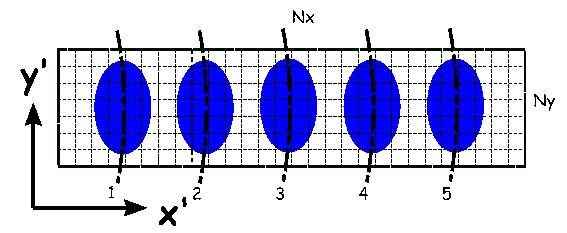
\includegraphics[width=60mm]{figures/SM-MultiBunch.ps}
  \caption{Schematic plot of the top view of 5 bunches and the grid of computation domain. The grid size on $X'-Y'$ plane is Nx$\times$Ny, and the broken lines represent the orbits of beam centroids. }
  \label{fig:MultiBunch}
\end{figure}

Here another question raises. How many bunches should be simulated to evaluate neighboring bunch effects?  
A pragmatic approach is given by doing the simulation for 3 bunches and 5 bunches and comparing phase space results first. If the discrepancy is visible, one needs to do 
the simulation for 7 bunches, and compare its result with 5 bunches, and so forth. 
Eventually, with the proper setting of $N_B$ and $M$, neighboring bunch effects can be evaluated precisely.
For instance, the setting with $N_B=9, M=4.5$ gives a convergent result for the PSI Ring cyclotron of 1\,mA beam current.
We will discuss this in more detail in the following section. 

In a multi-bunch simulation the energy of bunches in different turns is quite different. One can't find a single beam rest frame in which the relative motions of 
particles are sufficiently non-relativistic. Consequently it is not sufficient to use only one rest frame 
and a single Lorentz transformation. In order to calculate space charge fields more precisely, an adaptive energy binning technique is applied to improve 
the computational accuracy. 

\section{IMPLEMENTATION WITHIN THE \opal \  FRAMEWORK}

The above model and algorithm is implemented in the object-oriented parallel PIC code \opalcycl. 
\opalcycl \  is one of the flavors of the Object Oriented Parallel Accelerator Library (\opal) framework \cite{opal:1}. This framework is a powerful tool for charged-particle optics in general accelerator structures and beam lines.
Using the MAD languages with extensions,
\opal \  is derived from MAD9P \cite{Ada:1} and is based on the CLASSIC \cite{Classic:1} library and the Independent Parallel Particle Layer (IPPL) framework \cite{Ippl:1}. 
The CLASSIC library is a C++ class library which provides services for building portable accelerator models and algorithms and input 
language to specify complicated accelerator systems in general. IPPL is an Object-Oriented C++ class library which provides a flexible
environment for data-parallel programming of scientific application. It provides an integrated, layered system of objects. The upper layers
contain global data objects of physical/mathematical quantities, such as particles, fields and matrices of meshes and typical methods
performed on these objects such as binary operators and FFT. the lower layers contain the object's relevant to parallelization and efficient node-level
simulation, such as data distribution, domain decomposition and communication among processors, load balancing and chained-expression optimization. 
The intermediate phase space data of all particles and some interesting parameters, 
including RMS envelop size, RMS emittance, energy, path length, bunch numbers and 
tracking step, are stored in the H5Part \cite{H5part:1} file-format and can be analyzed
using the visualization tool H5PartRoot \cite{Thomas:1}.

In addition, apart from the multi-particle simulation mode, \opalcycl \  also has two other serial tracking modes for conventional cyclotron machine design. 
One mode is the single particle tracking mode, which is a useful tool for 
the preliminary design of a new cyclotron. It allows to compute  basic parameters, such as reference orbit, phase shift history,
stable region and matching phase ellipse. The other one is the tune calculation mode, which can be used to compute the betatron oscillation frequency 
$\nu_r$ and $\nu_z$. This is useful for evaluating 
the focusing characteristics of a given magnetic field map. 

A more detailed description of the hierarchical layout, the parallelization and the implementation issues of the \opal \  framework and \opalcycl \  code
can be found in the User's Reference Guide \cite{opal:1}.  

\section{APPLICATIONS}

\subsection{Different phase widths study of PSI Ring}

Although a very compact beam of about $2^\circ$ phase width can be extracted from the Injector 2 cyclotron, it expands in the longitudinal direction in the 72 MeV beam 
beam line because of space charge effects and chromatic dispersion. For the future 3\,mA beam, this will be even more pronounced and in consequence change the
Ring injection point in phase space.
A 10$th$ harmonic buncher is planed to be installed in the 72 MeV beam line to re-bunch the beam at injection of the Ring cyclotron.
Therefore, how short the bunch should be achieved at the injection point of the Ring is a critical question. 

In order to obtain a clear perspective on this issue, \opalcycl \  was applied to do numerical simulation on the Ring cyclotron by tracking 3
different initial conditions assuming a Gaussian beam at injection. The initial longitudinal phase widths (6$\sigma$) are set to $2^\circ$, $6^\circ$ and $10^\circ$, respectively,
and a Gaussian initial energy spread of 0.1\%. In the transverse and vertical directions the initial beam size (6$\sigma$) are set to 12\,mm. 
%On the horizontal direction, the beam sizes are $12$\,mm and momenta are set to zero. On the vertical direction, beam sizes and momenta are $12$\,mm and $3.4\times10^{-4}$. 
The initial distribution are assumed uncorrelated in phase space.
\begin{figure*}
  \centering
  \includegraphics*[width=0.45\linewidth]{figures/Comp-Transverse.ps}
  \includegraphics*[width=0.45\linewidth]{figures/Comp-Longitudinal.ps}
  \caption{Comparison of the rms beam size in the transverse direction (left) and longitudinal direction (right) at $112^\circ$ azimuthal position of each turn 
    in PSI Ring cyclotron. }
  \label{fig:RMSsize}
\end{figure*}

\begin{figure*}
  \centering
  \includegraphics*[angle=90,width=0.25\linewidth]{figures/Theta-Turn-0.ps}
  \includegraphics*[angle=90,width=0.25\linewidth]{figures/Theta-Turn-50.ps}
  \includegraphics*[angle=90,width=0.25\linewidth]{figures/Theta-Turn-150.ps}
  \caption{Longitudinal distribution of 3\,mA bunch distributions with  $2^\circ$, $6^\circ$ and $10^\circ$ initial phase widths at initial position (left), turn 50 (middle) and 150 (right) in PSI Ring cyclotron.}
  \label{fig:ThetaHitgram}
\end{figure*}

In Fig.\,\ref{fig:RMSsize} is shown the development of the beam rms size in transverse and the longitudinal directions. We can see the beam is compressed
gradually in the longitudinal direction. Meanwhile in the transverse direction, the beam size increases fast during the first several turn 
because of the mismatch of initial conditions. Thereafter it does not change sufficiently until the beam arrives at the last few turns 
where the beam experiences the fringe field.
Fig.\,\ref{fig:ThetaHitgram} plots the histogram along the longitudinal direction at $112^\circ$ azimuthal position of turn 0, 50 and 150.
The bunch with the initial phase width of $2^\circ$ maintains very compact shape with a stable round core and no halos at all. 
When the initial phase width increases, the size of core only widens for less than 5\,mm, but the spiral tails expands in the longitudinal direction and 
can't develop stable halos. However, the beam does not expands notably in radial direction, which means no substantial increase of the beam loss 
on the extraction septum is expected for the bunch with initial phase width less than $10^\circ$.

\subsection {Neighboring bunch effects in PSI Ring}

As described above, with the proper setting of $N_B$ (odd number, larger than 1) and $M$, 
space charge effects of both bunch itself and neighboring bunch effects can be included in \opalcycl simulation. 
Meanwhile, if only a single bunch is tracked, namely $N_B=1$, only space charge effects of bunch itself are included. 
Therefore one can evaluate the influence of neighboring bunch effects by comparing the results of these two kinds of simulation.
We did simulations with $M=4.5$ and $N_B=3, 5, 7, 9$, respectively. We found the simulations with $N_B=7$ and $N_B=9$ give out close results,
as shown the middle and right plots in Fig.\,\ref{fig:NBcompare2D}. 
This means the setting with $N_B=9, M=4.5$ gives a convergent result for the PSI Ring cyclotron of 1\,mA beam current.

We can see from Fig.\,\ref{fig:NBcompare}, the FWHD of beam transverse profile from multi-bunch simulation is about 1\,mm narrower than that of single bunch and that the FWHD of energy spread is reduced slightly. This is caused by squeezing space charge force from the bunches at the smaller radius 
and those at the bigger radius. 

From the comparison, we conclude that neighboring bunch effects impose visible impacts on the beam dynamics when the beam current get beyond 1\,mA in PSI Ring. 
The bunch becomes more compact in the transverse direction and the energy spread is reduced slightly. Therefore neighboring bunch effects have positive influence
on reducing beam loss in high intensity operation.

\begin{figure*}
  \centering
  \includegraphics[angle=90,width=1\linewidth]{figures/C9B7BSB-2D-1mA-130.ps}
  \caption{Top view of 1\,mA bunch distributions at the turn 130  in the local frame at $112^\circ$ azimuthal position of turn 130 in PSI Ring cyclotron.
    The results are obtained from single bunch (left), 7 bunches (middle) and 9 bunches (right) simulations, respectively.}
  \label{fig:NBcompare2D}
\end{figure*}

\begin{figure*}
  \centering
  \includegraphics[angle=90,width=80mm]{figures/C9B7BSB-R-1mA-130.ps}
  \includegraphics[angle=90,width=80mm]{figures/C9B7BSB-Energy-1mA-130.ps}
  \caption{Comparison of the histograms along the transverse direction in the local frame (left) and the energy spectra (right) of 1\,mA beam
    at $112^\circ$ azimuthal position of turn 130 in PSI Ring cyclotron.}
  \label{fig:NBcompare}
\end{figure*}

\section{CONCLUSIONS AND DISCUSSIONS}
In this paper, we presented a physical model for the beam dynamics in high intensity cyclotrons, which includes for the first time the space charge effects
of neighboring bunches in a self-consistent way. This model is implemented in an object-oriented three-dimensional parallel PIC code, 
as a flavor of the \opal\, framework. 

This code has been successfully applied to study the behavior of the PSI Ring cyclotron at high intensities.
As the results show, the generation of beam tails can be avoided if short bunches with a phase length of $2^\circ$  or less are injected. 
An upgrade plan is under way to generate such short bunches with the help of a 10$th$ harmonic buncher.
Furthermore it is observed that the neighboring bunch effects can help to narrow the transverse beam size and reduce the energy spread.

It is planned to refine these simulations within the next year by a more detailed determination of the initial particle distribution at the injection
of the PSI Ring cyclotron. A quantitative comparison of the results with measured beam properties will be presented in a future paper.
%Perform the first parallel simulation of multiple bunches in cyclotron
%Study neighboring bunch effects on the beam's evolution quantitatively on PSI Ring cyclotron
\section{ACKNOWLEDGMENTS}
The authors thank the AMAS grop members C.\,Kraus, Y.\,Ineichen and B.\,Oswald for many 
discussions regarding programming and T.\,Schietinger for providing the post-processing tool
H5PartRoot. We also thank W.\,Joho, S.\,Adam and R.\,Doelling for many useful discussions regarding high
intensity beam dynamics in cyclotrons. This work was performed on the Merlin3 cluster at Paul Scherrer Institut 
and Cray XT3 at Swiss National Supercomputing Center (CSCS). 


\begin{thebibliography}{99}   % Use for  10-99  references

\bibitem{Gordon:1}
  M. M. Gordon, in Proc. 5th Int. Conf. on Cyclotrons and their Applications, Oxford, (1969), p. 305.
\bibitem{Joho:1}
  W. Joho, in Proc. 9th Int. Conf. on Cyclotrons and their Applications, Caen, (1981), p. 337.
\bibitem{Adam:1}
  S. Adam, IEEE Trans. on Nuclear Science 32, (1985) p. 2507.
\bibitem{Adam:2}
  S. Koscielniak and S. Adam, in Proc. Particle Accelerator Conf., Washington, (1993), p. 3639.
\bibitem{Ada:1}
  A. Adelmann, Ph.D. thesis, ETHZ, Switzerland (2002), 14545.
\bibitem{Mike:1}
  M. Seidel and P. Schmelzbach, in Proc. 18th Int. Conf. on Cyclotrons and their Applications, Catania, (2007), p. 157.
\bibitem{Poz:1}
  E. Pozdeyev, Ph.D. thesis, MSU, USA (2003).
\bibitem{opal:1}
  A. Adelmann, Y. Ineichen, C. Kraus, S. Russell, and J. Yang, Tech. Rep. PSI-PR-08-02, Paul Scherrer Institut (2008).
\bibitem{Classic:1}
  F. Iselin, in Comput. Accelerator Physics Conf., Williamsburg, (1996).
\bibitem{H5part:1}
  A. Adelmann, R. Ryne, J. Shalf, and C. Siegerist, in Proc. Particle Accelerator Conf., Knoxville, (1999).
\bibitem{Thomas:1}
  http://amas.web.psi.ch/ tools/H5PartROOT/index.html
\bibitem{Ippl:1}
  http://amas.web.psi.ch/ tools/
\end{thebibliography}
\end{document}
